%<<<1 Header
\documentclass[xcolor=x11names,10pt]{beamer}

% This is the header file I usually use in my presentations

\usepackage{tikz,amsmath,bbold,cmbright}

\usetikzlibrary[positioning,arrows,arrows.meta,shapes,calc,spy,intersections,shadows]
\usetikzlibrary[decorations.text,decorations.pathmorphing,decorations.markings]

\parindent 0pt
\beamertemplatenavigationsymbolsempty
\usebackgroundtemplate{%
\tikz\fill[white] (0,0) to (\paperwidth,\paperheight);}
\geometry{left=0in,top=-0.015in,right=0in,bottom=0.0in}
\renewcommand\b\mathbold
\renewcommand\d{{\sf d}}

% main slide picture
\newcommand{\mypic}[2]{%
  \begin{tikzpicture}[remember picture,
      x=0.01\paperwidth,y=0.01\paperheight,
      title/.style={anchor=base,scale=1.5,font=\bfseries,text=black},
      #1]{
  \draw [white] (0,0) rectangle (100,100);
  \begin{scope}
  \clip (0,0) rectangle (100,100);
  #2
  \end{scope}
  }
\end{tikzpicture}}

\setbeamercolor{itemize item}{fg=black}  

\newcommand{\outline}[3]{
  \begin{frame}
    \mypic{}{
    \node at (50, 90)[title] {Outline};
    \node[text width = 0.8\paperwidth, align=left, anchor=north west] at (#1, #2){
    \tableofcontents[#3]
    };}
  \end{frame}
}


\newcommand{\bibcreate}[1]{\addbibresource{#1.bib} \bibliographystyle{plain} \bibliography{#1}}


\setbeamerfont{section in toc}{size=\large,series=\bfseries}
\setbeamerfont{subsection in toc}{size=\large,series=\mdseries}
%\setlength{\parskip}{5em}
%\setbeamertemplate{section in toc}[square]  % Changes section bullet style
%\setbeamertemplate{subsection in toc}[circle] 

\setbeamertemplate{section in toc}{%
  \vspace{1em}
  \inserttocsection
  }

\usepackage{comment,bm}

% you might want to define colours here
%\definecolor{exc}{HTML}{E51E10}
%\definecolor{inh}{HTML}{56B4E9}



\begin{document}


%<<<1 Title
\begin{frame}
\mypic{}{   

\node (title) at (50,92) [below,scale=2,font=\bfseries,align=center,
  inner sep=1em] {
  RT Modelling with RNNs (and more)};

\node (author) at (50,60) [font=\bfseries] {Tim Lin};

  %\draw[xstep=1,ystep=1,color=gray!20] (0,0) grid (100,100);  
\draw[xstep=5,ystep=5,color=gray!60] (0,0) grid (100,100);  
\foreach \j in {10,20,...,90} \node at (2,\j) {\tiny{\j}};
\foreach \j in {10,20,...,90} \node at (98,\j) {\tiny{\j}};
\foreach \j in {10,20,...,90} \node at (\j,98) {\tiny{\j}};
\foreach \j in {10,20,...,90} \node at (\j,2) {\tiny{\j}};



\coordinate (logos) at (50,2);
\node at (20, 15) [center]
  {\includegraphics[width=8em]{figs/princeton.png}};
\node at (50, 15) [center]
  {\includegraphics[width=8em, trim=400 120 400 120, clip]{
  figs/nyu.png
  }};
\node (email) [below=0em of author.south] {\texttt{yl0124@princeton.edu}};
\node (context) [below=0em of email.south] {\today};

}
\end{frame}

%<<<1 Empty new slide with grid
\section{Task to model}%
  \label{sec:Task to model}

\begin{frame}
  \mypic{}{
  \node at (50,92) [anchor=base,title] {Task to model};
  \node at (10,83) [anchor = north west]{Behavioral Task}; 

  \node at (50, 68)[anchor = center] {
  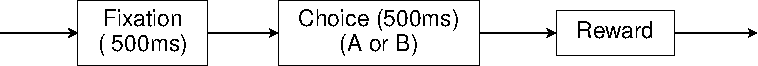
\includegraphics[width = 0.8\textwidth]{figs/task.pdf}
  };
  \node at (10,55) [anchor = north west]{Modelling Abstraction}; 

  \node at (50,25)[anchor = center] {
  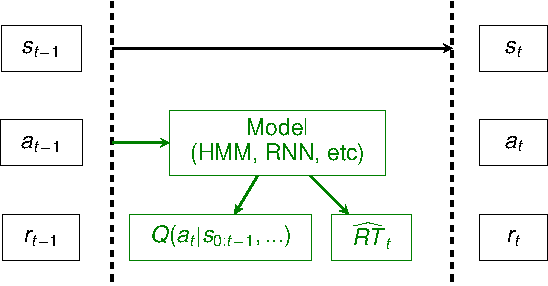
\includegraphics[width = 0.6\textwidth]{figs/model_abstract.pdf}
  };
  }
  
\end{frame}

\section{Modelling Approaches}%
  \label{sec:Modelling Approaches}


\outline{10}{80}{currentsection}

\begin{frame}
  \mypic{}{
  \node at (50,92) [anchor=base,title] {Modelling Approaches};
  %\draw[xstep=1,ystep=1,color=gray!20] (0,0) grid (100,100);  
\draw[xstep=5,ystep=5,color=gray!60] (0,0) grid (100,100);  
\foreach \j in {10,20,...,90} \node at (2,\j) {\tiny{\j}};
\foreach \j in {10,20,...,90} \node at (98,\j) {\tiny{\j}};
\foreach \j in {10,20,...,90} \node at (\j,98) {\tiny{\j}};
\foreach \j in {10,20,...,90} \node at (\j,2) {\tiny{\j}};




  \node  [anchor = north west, align = left, text width = 0.8\paperwidth] at (10, 83) { 
  \textbf{Making Choice and RT predictions} \\ 
  \vspace{1em}
  \begin{itemize}
    \item RTified RNN 
    \item RT RNN (Generalized RTified RNN)
  \end{itemize}\\
  \vspace{1em}
  Output: \texttt{choice\_pred} $\in [0,1]^{T \times 2}$, \texttt{rt\_pred} $\in \mathbb{R}_+^{T}$\\
  \vspace{2em}

  \textbf{Modelling the entire decision-making trajectory}\\
  \vspace{1em}
  \begin{itemize}
    \item Finite-state Automata 
    \item Time-discretized RNN \
  \end{itemize}
  \vspace{1em}
  Output: \texttt{action\_pred} $ \in [0,1]^{T \times 3}$ (hold, left, right)
  };
  }
  
\end{frame}



\subsection{RNN Models}%
  \label{sub:RNN Models}
  

\begin{frame}
  \mypic{}{
  %\draw[xstep=1,ystep=1,color=gray!20] (0,0) grid (100,100);  
\draw[xstep=5,ystep=5,color=gray!60] (0,0) grid (100,100);  
\foreach \j in {10,20,...,90} \node at (2,\j) {\tiny{\j}};
\foreach \j in {10,20,...,90} \node at (98,\j) {\tiny{\j}};
\foreach \j in {10,20,...,90} \node at (\j,98) {\tiny{\j}};
\foreach \j in {10,20,...,90} \node at (\j,2) {\tiny{\j}};



  \node at (50,92) [anchor=base,title] {RTified RNN (factorized)};
  \node at (10, 83) [anchor = north west, text width = 0.8\paperwidth, align = left]{
  Model: 
  };
  \node at (50, 79) [text width = 0.8\paperwidth, anchor = north]{
  \begin{align}
    \textbf{h}^{\text{slow}}_0 &\sim  \mathcal{N}(0, I) \notag\\
    \textbf{h}^{\text{slow}}_{1:\text{trials}} &= \text{RNN}^{\text{slow}}(\textbf{h}_{0:\text{trials}-1}, \textbf{u}_{1:\text{trials}}) \notag\\
    \hat{\textbf{x}}_{i}^{\text{choice}} &= \text{MLP}^{\text{choice}}(\textbf{h}^{slow}_{i}) \notag\\
    \textbf{h}^{\text{fast}}_{0, i} & = \text{MLP}^{\text{init}}(\textbf{h}^{\text{slow}}_{i}) \notag\\
    \textbf{h}^{\text{fast}}_{1:S, i} &= \text{RNN}^{\text{fast}}(\textbf{h}^{\text{fast}}_{0:S-1, i}, \textbf{u}_{1:S, i}) 
    \notag
    \\
    \hat{\textbf{x}}_{i}^{\text{RT}} &= \tau(\Phi(\textbf{h}_{1:S, i}^{\text{fat}}), \theta) \notag
  \end{align}
  };

  \node at (10, 35) [anchor = north west, text width = 0.8\paperwidth, align = left]{
  Loss: };
  \node at (50, 32) [text width = 0.8\paperwidth, anchor = north]{
  \begin{align}
    \mathcal{L} &= \left \langle \sum_{i=1}^{\text{trials}} \text{CE}(\textbf{x}_i ^{\text{choice}}, \hat{\textbf{x}}_i ^{choice})
    + \lambda_\text{RT} \text{MSE}(\textbf{x}_i ^{\text{RT}}, \hat{\textbf{x}}_i ^{RT})
    \right \rangle_{\text{batch}} \notag
  \end{align}
  };
  }
\end{frame}

\begin{frame}
  \mypic{}{
  %\draw[xstep=1,ystep=1,color=gray!20] (0,0) grid (100,100);  
\draw[xstep=5,ystep=5,color=gray!60] (0,0) grid (100,100);  
\foreach \j in {10,20,...,90} \node at (2,\j) {\tiny{\j}};
\foreach \j in {10,20,...,90} \node at (98,\j) {\tiny{\j}};
\foreach \j in {10,20,...,90} \node at (\j,98) {\tiny{\j}};
\foreach \j in {10,20,...,90} \node at (\j,2) {\tiny{\j}};



  \node at (50,92) [anchor=base,title] {RTified RNN (shared)};
  \node at (10, 83) [anchor = north west, text width = 0.8\paperwidth, align = left]{
  $T$ : $\text{trials} \times S$.  

  \vspace{1em}

  Model: 
  };
  \node at (50, 74) [text width = 0.8\paperwidth, anchor = north]{
  \begin{align}
    \textbf{h}_0 &\sim  \mathcal{N}(0, I) \notag\\
    \textbf{h}_{1:T} &= \text{RNN}(\textbf{h}_{0:T-1}, \textbf{u}_{1:T}) \notag\\
    \hat{\textbf{x}}_{i}^{\text{choice}} &= \text{MLP}^{\text{choice}}(\textbf{h}_{Si + 1: Si + S}) \notag\\
    \hat{\textbf{x}}_{i}^{\text{RT}} &= \tau(\Phi(\textbf{h}_{Si + 1: Si + S}), \theta) \notag
  \end{align}
  };

%  \begin{align}
%    \textbf{h}^{\text{slow}}_0 &\sim  \mathcal{N}(0, I) \notag\\
%    \textbf{h}^{\text{slow}}_{1:\text{trials}} &= \text{RNN}^{\text{slow}}(\textbf{h}_{0:\text{trials}-1}, \textbf{u}_{1:\text{trials}}) \notag\\
%    \hat{\textbf{x}}_{i}^{\text{choice}} &= \text{MLP}^{\text{choice}}(\textbf{h}^{slow}_{i}) \notag\\
%    \textbf{h}^{\text{fast}}_{0, i} & = \text{MLP}^{\text{init}}(\textbf{h}^{\text{slow}}_{i}) \notag\\
%    \textbf{h}^{\text{fast}}_{1:S, i} &= \text{RNN}^{\text{fast}}(\textbf{h}^{\text{fast}}_{0:S-1, i}, \textbf{u}_{1:S, i}) 
%    \notag
%    \\
%  \end{align}
%  };

  \node at (10, 35) [anchor = north west, text width = 0.8\paperwidth, align = left]{
  Loss: };
  \node at (50, 32) [text width = 0.8\paperwidth, anchor = north]{
  \begin{align}
    \mathcal{L} &= \left \langle \sum_{i=1}^{\text{trials}} \text{CE}(\textbf{x}_i ^{\text{choice}}, \hat{\textbf{x}}_i ^{choice})
    + \lambda_\text{RT} \text{MSE}(\textbf{x}_i ^{\text{RT}}, \hat{\textbf{x}}_i ^{RT})
    \right \rangle_{\text{batch}} \notag
  \end{align}
  };
  }
\end{frame}


\begin{frame}
  \mypic{}{
  %\draw[xstep=1,ystep=1,color=gray!20] (0,0) grid (100,100);  
\draw[xstep=5,ystep=5,color=gray!60] (0,0) grid (100,100);  
\foreach \j in {10,20,...,90} \node at (2,\j) {\tiny{\j}};
\foreach \j in {10,20,...,90} \node at (98,\j) {\tiny{\j}};
\foreach \j in {10,20,...,90} \node at (\j,98) {\tiny{\j}};
\foreach \j in {10,20,...,90} \node at (\j,2) {\tiny{\j}};



  \node at (50,92) [anchor=base,title] {RT RNN (shared)};
  \node at (10, 83) [anchor = north west, text width = 0.8\paperwidth, align = left]{
  Model: 
  };
  \node at (50, 79) [text width = 0.8\paperwidth, anchor = north]{
  \begin{align}
    \textbf{h}_0 &\sim  \mathcal{N}(0, I) \notag\\
    \textbf{h}_{1:T} &= \text{RNN}(\textbf{h}_{0:T-1}, \textbf{u}_{1:T}) \notag\\
    \hat{\textbf{x}}_{i}^{\text{choice}} &= \text{MLP}^{\text{choice}}(\textbf{h}_{Si: Si + S}) \notag\\
    \hat{\textbf{x}}_{i}^{\text{RT}} &= \color{red}{\text{MLP}^{\text{RT}}(\textbf{h}_{Si: Si + S})}\notag
  \end{align}
  };

  \node at (10, 45) [anchor = north west, text width = 0.8\paperwidth, align = left]{
  Loss: };
  \node at (50, 42) [text width = 0.8\paperwidth, anchor = north]{
  \begin{align}
    \mathcal{L} &= \left \langle \sum_{i=1}^{\text{trials}} \text{CE}(\textbf{x}_i ^{\text{choice}}, \hat{\textbf{x}}_i ^{choice})
    + \lambda_\text{RT} \text{MSE}(\textbf{x}_i ^{\text{RT}}, \hat{\textbf{x}}_i ^{RT})
    \right \rangle_{\text{batch}} \notag
  \end{align}
  };
  }
\end{frame}

\begin{frame}
  \mypic{}{
  %\draw[xstep=1,ystep=1,color=gray!20] (0,0) grid (100,100);  
\draw[xstep=5,ystep=5,color=gray!60] (0,0) grid (100,100);  
\foreach \j in {10,20,...,90} \node at (2,\j) {\tiny{\j}};
\foreach \j in {10,20,...,90} \node at (98,\j) {\tiny{\j}};
\foreach \j in {10,20,...,90} \node at (\j,98) {\tiny{\j}};
\foreach \j in {10,20,...,90} \node at (\j,2) {\tiny{\j}};



  \node at (50,92) [anchor=base,title] {Time-discretized RNN};
  \node at (10, 83) [anchor = north west, text width = 0.8\paperwidth, align = left]{
  Instead of turning "discretized-trajectories" into RT and choice predictions, use RT to reconstruct the entire trial trajectory. 

  \vspace{1em}

  Ask the model to reconstruct the entire trial trajectory $\textbf{x}_{1 : T}$ given control inputs (that the subject received) $\textbf{u}_{1 : T}$, where $T$ is the total number of discretized time steps across all trials.

  \vspace {1em}
  
  \begin{itemize}
    \item Separation of different sub-trial events; dissect phase-planes and fixed-point structures. 
    \item Direct interpretability of the model's internal dynamics. Amenable to joint behavioral-neural data modelling. 
    \color{red}{\item Extra model complexity needed (empirically show this and comment on parameter retrieval)}\footnote{we don't necessarily care so much about the evidence accumulation in classical cognitive model settings?}\footnote{also RNNs, where inputs come in additively, are not necessarily the most appropriate models here.}
  \end{itemize}
  };
  }
\end{frame}


\begin{frame}
  \mypic{}{
  %\draw[xstep=1,ystep=1,color=gray!20] (0,0) grid (100,100);  
\draw[xstep=5,ystep=5,color=gray!60] (0,0) grid (100,100);  
\foreach \j in {10,20,...,90} \node at (2,\j) {\tiny{\j}};
\foreach \j in {10,20,...,90} \node at (98,\j) {\tiny{\j}};
\foreach \j in {10,20,...,90} \node at (\j,98) {\tiny{\j}};
\foreach \j in {10,20,...,90} \node at (\j,2) {\tiny{\j}};



  \node at (50,92) [anchor=base,title] {Time-discretization Example};
  \node at (10, 83) [anchor = north west, text width = 0.8\paperwidth, align = left]{
  Example $\textbf{u}$ within a trial: 
  };
  \node at (28, 70) [anchor = north]{
  \includegraphics[width = 0.4\textwidth] {../../figures/input_features_example.png}
  };
  \node at (54, 83) [anchor = north west, text width = 0.8\paperwidth, align = left]{
  Example $\textbf{x}$ within a trial \\(gaussian-smoothed): 
  };
  \node at (75, 70) [anchor = north]{
  \includegraphics[width = 0.4\textwidth] {../../figures/output_example.png}
  };
  }
\end{frame}

\begin{frame}
  \mypic{}{
  %\draw[xstep=1,ystep=1,color=gray!20] (0,0) grid (100,100);  
\draw[xstep=5,ystep=5,color=gray!60] (0,0) grid (100,100);  
\foreach \j in {10,20,...,90} \node at (2,\j) {\tiny{\j}};
\foreach \j in {10,20,...,90} \node at (98,\j) {\tiny{\j}};
\foreach \j in {10,20,...,90} \node at (\j,98) {\tiny{\j}};
\foreach \j in {10,20,...,90} \node at (\j,2) {\tiny{\j}};



  \node at (50,92) [anchor=base,title] {Time-discretized RNN};

  \node at (10, 83) [anchor = north west, text width = 0.8\paperwidth, align = left]{
  Model: 
  };
  \node at (50, 79) [text width = 0.8\paperwidth, anchor = north]{
  \begin{align}
    \textbf{h}_0 &\sim  \mathcal{N}(0, I) \notag\\
    \textbf{h}_{1:T} &= \text{RNN}(\textbf{h}_{0:T-1}, \textbf{u}_{1:T}) \notag\\
    \textbf{x}_{1:T} &= \text{MLP}(\textbf{h}_{1:T}) \notag
  \end{align}
  };

  \node at (10, 45) [anchor = north west, text width = 0.8\paperwidth, align = left]{
  Loss: };
  \node at (50, 42) [text width = 0.8\paperwidth, anchor = north]{
  \begin{align}
    \mathcal{L} &= \left \langle \sum_{t=1}^{T} \text{CE}(\textbf{x}_t, \textbf{x}_t)\right \rangle_{\text{batch}} \notag
  \end{align}
  };
  }
\end{frame}

\begin{frame}
  \mypic{}{
  %\draw[xstep=1,ystep=1,color=gray!20] (0,0) grid (100,100);  
\draw[xstep=5,ystep=5,color=gray!60] (0,0) grid (100,100);  
\foreach \j in {10,20,...,90} \node at (2,\j) {\tiny{\j}};
\foreach \j in {10,20,...,90} \node at (98,\j) {\tiny{\j}};
\foreach \j in {10,20,...,90} \node at (\j,98) {\tiny{\j}};
\foreach \j in {10,20,...,90} \node at (\j,2) {\tiny{\j}};



  \node at (50,92) [anchor=base,title] {Time-discretization RNN Trained Result};
  \node at (10, 83) [anchor = north west, text width = 0.8\paperwidth, align = left]{
  Example $\textbf{x}$ vs. $\hat{\textbf{x}}$ (taken from one trial sequence)
  };
  \node at (50, 75) [anchor = north]{
  \includegraphics[width = 0.9\textwidth] {../../figures/discretised_rnn_output_example_pad_ones.png}
  };
  }
\end{frame}

\begin{frame}
  \mypic{}{
  %\draw[xstep=1,ystep=1,color=gray!20] (0,0) grid (100,100);  
\draw[xstep=5,ystep=5,color=gray!60] (0,0) grid (100,100);  
\foreach \j in {10,20,...,90} \node at (2,\j) {\tiny{\j}};
\foreach \j in {10,20,...,90} \node at (98,\j) {\tiny{\j}};
\foreach \j in {10,20,...,90} \node at (\j,98) {\tiny{\j}};
\foreach \j in {10,20,...,90} \node at (\j,2) {\tiny{\j}};



  \node at (50,92) [anchor=base,title] {Time-discretization RNN Trained Result 2};
  \node at (10, 83) [anchor = north west, text width = 0.8\paperwidth, align = left]{
  Example $\langle\textbf{x}, \hat{\textbf{x}}\rangle$, averaged across vs. within trials. 
  };
  \node at (50, 68) [anchor = north]{
  \includegraphics[width = 0.9\textwidth] {../../figures/discretised_rnn_dot_product_pad_ones.png}
  };
  }
\end{frame}

\subsection{Finite-state Automata}%
\label{sub:Finite-state Automata}

\begin{frame}

  \mypic{}{
  \node at (50,92) [anchor=base,title] {Finite-state Automata};
  %\draw[xstep=1,ystep=1,color=gray!20] (0,0) grid (100,100);  
\draw[xstep=5,ystep=5,color=gray!60] (0,0) grid (100,100);  
\foreach \j in {10,20,...,90} \node at (2,\j) {\tiny{\j}};
\foreach \j in {10,20,...,90} \node at (98,\j) {\tiny{\j}};
\foreach \j in {10,20,...,90} \node at (\j,98) {\tiny{\j}};
\foreach \j in {10,20,...,90} \node at (\j,2) {\tiny{\j}};



  \node at (50, 92) [anchor = north]{
  \includegraphics[trim = 80 80 30 60, clip, width = 0.7\textwidth]{
../../figures/hmm_vis.png
  }
  };
  }
\end{frame}
\begin{frame}
  \mypic{}{
  \node at (50,92) [anchor=base,title] {SFSA Model Appendix (credits to Prakhar)};
  \node at (50,88) [anchor = north, text width = 0.8\paperwidth, align = left]{
The sequential decision setting, e.g. n-armed Bernoulli bandit.
The (time-dependent) decision function / policy based on stochastic finite state automaton defined as follows:
\\
Let there be given some environment with:
\begin{itemize}
    \item $S$ a finite set of environment states;
    \item $A$ a finite set of actions that an agent can take, with $\bar{A} = A \cup \{*\}$, where `$*$' represents the empty action;
    \item $T$ a probabilistic transition $S \times \bar{A} \to S$, such that for all $a \in \bar{A}$, $T_a \in \RR^{S \times S}$ is a probability matrix.
\end{itemize}
\paragraph*{Bandit Example.} The environment can be an iterated $n$-armed Bernoulli bandit. Here, the environment states would be the outcomes of pulling an arm, e.g. $S = {0,1}$, and the actions would be the $n$ arms.
The bandit environment provides for any arm $a \in \bar{A}$ chosen, a probability $p_a$, such that the follow-up state is $1$ with probability $p_a$ and to $0$ with probability $1-p_a$. If the empty action $* \in \bar{A}$ is chosen, then the state changes to $0$ with probability $1$, i.e., $p_* = 0$. In the bandit case, the current state has not effect on the transition probabilities.
  };}
\end{frame}

\begin{frame}
  \mypic{}{
  \node at (50,95) [anchor = north, text width = 0.8\paperwidth, align = left]{
Let $(\Omega, Q, \{P_o\}_{o \in \Omega})$ be a probabilistic automaton, where
%
\begin{itemize}
    \item $\Omega$ is a partition of $\bar{A} \times S$ denoting the set of inputs for the automaton; e.g., in an $n$-armed bandit setting this might be a set of tuples representing an action taken and the \emph{resulting} environment state; in a more general setting, one might require that $\Omega$ is a partition of $S \times \bar{A} \times S$; for notational simplicity, we assume $\Omega$ to be the finest partition and simplify to $\Omega = \bar{A} \times S$;
    \item $Q$ is a finite set of states;
    \item for $\omega \in \Omega$, $P_\omega$ is a right-stochastic matrix such that for any $q, q' \in S$, $[P_\omega]_{qq'}$ is the probability for a transition from state $q$ to $q'$ under input $\omega$, i.e. for $q \overset{\omega}{\rightarrow} q'$.
\end{itemize}
Let further
\begin{itemize}
    \item $\pi: Q \rightarrow D(\bar{A})$ be the probabilistic action readout, where $D(\bar{A})$ is the set of probability distributions over $\bar{A}$, yielding for any given automaton state either an actual action or the empty action;
    \item $R: \Omega \to \RR$ be the agent's/automaton's reward function.
\end{itemize} }; }
\end{frame}

\begin{frame}
  \mypic{}{
  \node at (50,95) [anchor = north, text width = 0.8\paperwidth, align = left]{
\paragraph*{Conditional Transitions.}
The resulting stochastic process then looks as follows
 
$ \ldots \to a_{t-1} \to s_t \to q_t \to a_t \to s_{t+1} \to q_{t+1} \to a_{t+1} \to s_{t+2} \ldots $

  \vspace{1em}
and the conditional transitions look as follows: 
  
\begin{align}
%
\Pr( s_{t+1} = s' | s_t, q_t )
%& = \Pr( s_t \to s' | q_t )
%\\ & \quad
  &= \sum_{a \in \bar{A}} \Pr(a_t = a | q_t) \Pr(s_{t+1} = s' | s_t, a )
\notag\\
& = \sum_{a \in \bar{A}} \pi_{q_t}(a) T( (s_t, a) \to s' ) = \sum_{a \in \bar{A}} \pi_{q_t}(a) [T_a]_{s_t s'}
\notag\\
\Pr( q_{t+1} = q' | s_t, q_t )
%& = \Pr( q_t \to q' | s_t )
%\\ & \quad
  &= \sum_{a \in \bar{A}} \Pr(a_t = a | q_t) \sum_{s' \in S} \Pr(s_{t+1} = s' | (s_t, a) ) [P_{a,s'}]_{q_t q'}
\notag\\
%& \quad = \sum_{s' \in S} \sum_{a \in \bar{A}} \Pr(a_t = a | q_t) \Pr(s_{t+1} = s' | (s_t, a) ) [P_{a,s'}]_{q_t q'}
%\\
& = \sum_{s' \in S} \sum_{a \in \bar{A}} \pi_{q_t}(a) T( (s_t, a) \to s' ) [P_{a,s'}]_{q_t q'}\notag\\
%\\ & \quad
&= \sum_{s' \in S} \sum_{a \in \bar{A}} \pi_{q_t}(a) [T_a]_{s_t s'} [P_{a,s'}]_{q_t q'} \notag
\end{align}}; }
\end{frame}
\begin{frame}
  \mypic{}{
  \node at (50,92) [anchor=base,title] {Conditional Transitions (contd.)};
  %\draw[xstep=1,ystep=1,color=gray!20] (0,0) grid (100,100);  
\draw[xstep=5,ystep=5,color=gray!60] (0,0) grid (100,100);  
\foreach \j in {10,20,...,90} \node at (2,\j) {\tiny{\j}};
\foreach \j in {10,20,...,90} \node at (98,\j) {\tiny{\j}};
\foreach \j in {10,20,...,90} \node at (\j,98) {\tiny{\j}};
\foreach \j in {10,20,...,90} \node at (\j,2) {\tiny{\j}};



  \node at (50,92) [anchor = north, text width = 0.8\paperwidth, align = left]{

\begin{align}
\Pr( s_{t+1} = s', q_{t+1} =& q' | s_t = s, q_t = q ) \notag\\
%& = \Pr( s, q \to s', q' )
%\\ & \quad
&= \sum_{a \in \bar{A}} \pi_q(a) T( (s,a) \to s' ) [P_{a,s'}]_{q q'} \notag\\
& = \sum_{a \in \bar{A}} \pi_q(a) [T_a]_{s s'} [P_{a,s'}]_{q q'}  =: [M]_{(s,q),(s',q')}\notag\\
%& \quad = \sum_{s' \in S} \sum_{a \in \bar{A}} \Pr(a_t = a | q_t) \Pr(s_{t+1} = s' | (s_t, a) ) [P_{a,s'}]_{q_t q'}
%\\
%
%
\Pr( a_{t+1} = a' | s_t, q_t )
& = \sum_{q' \in Q} \Pr(q_t \to q' | s_t ) \Pr(a_{t+1} = a' | q') \notag\\ 
%\\ & \quad
  &= \sum_{q' \in Q} \Pr(q_t \to q' | s_t ) \pi_{q'}(a') \notag
% \\
% %
% \omega_{t+1}(a,1) & = P( (a_{t+1}, r_{t+1}) = (a,1) ) \\
%   & = p_a \sum_{q \in Q} \sigma_t(q) \pi_a(q)
% \\
% %
% \omega_{t+1}(a,0) & = P( (a_{t+1}, r_{t+1}) = (a,0) ) \\
%   & = (1-p_a) \sum_{q \in Q} \sigma_t(q) \pi_a(q)
\end{align}}; } 

\end{frame}
\begin{frame}
  \mypic{}{
  \node at (50,92) [anchor=base,title] {Stationarity and Evolution of Probabilities};
  %\draw[xstep=1,ystep=1,color=gray!20] (0,0) grid (100,100);  
\draw[xstep=5,ystep=5,color=gray!60] (0,0) grid (100,100);  
\foreach \j in {10,20,...,90} \node at (2,\j) {\tiny{\j}};
\foreach \j in {10,20,...,90} \node at (98,\j) {\tiny{\j}};
\foreach \j in {10,20,...,90} \node at (\j,98) {\tiny{\j}};
\foreach \j in {10,20,...,90} \node at (\j,2) {\tiny{\j}};



  \node at (50,88) [anchor = north, text width = 0.8\paperwidth, align = left]{
Overall, due to the stationary of the transitions, we have for all $h,t \in \NN_0$:
\begin{align*}
    & \Pr( s_{h+t} = s', q_{h+t} = q' | s_h = s, q_h = q ) = [M^t]_{(s,q),(s',q')} \\
    & \quad = \Pr( s_{t} = s', q_{t} = q' | s_0 = s, q_0 = q )   \label{eq:stationary}\tag{$*$}
\end{align*}
%At any time $t \in \NN$ the state of the whole system is a random variable $(s_t, q_t, a_t)$. The resulting process then looks as follows:
%
%
\paragraph*{Evolution of Probabilities.}
Given
a probability distribution $\rho_t$ over states $Q$, and
a probability distribution $\sigma_t$ over environment states $S$
%a probability distribution $\omega_t$ over inputs $\Omega$
at some time $t$, we have:
%
\begin{align*}
\sigma_{t+1}(s') & = \Pr( s_{t+1} = s' | \sigma_t, \rho_t )
  = \sum_{s \in S} \sum_{q \in Q} \sigma_t(s) \rho_t(q) \Pr(s \to s' | q)
\\
%
\rho_{t+1}(q') & = \Pr( q_{t+1} = q' | \sigma_t, \rho_t )
  = \sum_{s \in S} \sum_{q \in Q} \sigma_t(s) \rho_t(q) \Pr(q \to q' | s)
\\
  &\qquad \text{ for $s' \in S, q' \in Q$.}
%
\end{align*}
\paragraph*{Sequence of Rewards.}
From this, we have the sequence of rewards $\{R_t\}_{t \in \NN}$ with $R_t = R(a_{t-1},s_t)$, with suitable choice for $t = 0$, e.g., $R_t = 0$.
  };
  }
  
\end{frame}
  %%% -------------------------------------------------------
%\begin{frame}
%\mypic{}{   
%\node at (50,92) [anchor=base,title] {Slide title};
%
%\draw[xstep=1,ystep=1,color=gray!20] (0,0) grid (100,100);  
\draw[xstep=5,ystep=5,color=gray!60] (0,0) grid (100,100);  
\foreach \j in {10,20,...,90} \node at (2,\j) {\tiny{\j}};
\foreach \j in {10,20,...,90} \node at (98,\j) {\tiny{\j}};
\foreach \j in {10,20,...,90} \node at (\j,98) {\tiny{\j}};
\foreach \j in {10,20,...,90} \node at (\j,2) {\tiny{\j}};



%
%}
%\end{frame}
%
%<<<1 End
\end{document}

